

\documentclass[
	11pt, % Set the default font size, options include: 8pt, 9pt, 10pt, 11pt, 12pt, 14pt, 17pt, 20pt
	%t, % Uncomment to vertically align all slide content to the top of the slide, rather than the default centered
	%aspectratio=169, % Uncomment to set the aspect ratio to a 16:9 ratio which matches the aspect ratio of 1080p and 4K screens and projectors
]{beamer}

\graphicspath{{~/Pictures/}{./}} % Specifies where to look for included images (trailing slash required)

\usepackage{booktabs} % Allows the use of \toprule, \midrule and \bottomrule for better rules in tables
\usetheme{Madrid}
\usefonttheme{default} % Typeset using the default sans serif font
\usepackage{palatino} % Use the Palatino font for serif text
\usepackage[default]{opensans} % Use the Open Sans font for sans serif text
\useinnertheme{circles}
\title[SO classification with CNN]{Exploring CNNs for Space Object Classification}

%subtitle{Exploring CNNs for Space Object Classification} % Presentation subtitle, remove this command if a subtitle isn't required

\author[Hunsberger \and Cotton]{Carson Hunsberger \and Nicholas Cotton} % Presenter name(s), the optional parameter can contain a shortened version to appear on the bottom of every slide, while the main parameter will appear on the title slide
\date[\today]{\today} % Presentation date or conference/meeting name, the optional parameter can contain a shortened version to appear on the bottom of every slide, while the required parameter value is output to the title slide
\begin{document}
\begin{frame}
	\titlepage % Output the title slide, automatically created using the text entered in the PRESENTATION INFORMATION block above
\end{frame}
\begin{frame}
	\frametitle{Presentation Overview} % Slide title, remove this command for no title
	
	\tableofcontents % Output the table of contents (all sections on one slide)
	%\tableofcontents[pausesections] % Output the table of contents (break sections up across separate slides)
\end{frame}
\section{Introduction} % Sections are added in order to organize your presentation into discrete blocks, all sections and subsections are automatically output to the table of contents as an overview of the talk but NOT output in the presentation as separate slides
\subsection{What is a Space Object?}

\begin{frame}
	\frametitle{What is a Space Object?}
	\begin{itemize}
		\item
			A Space Object(SO) is any entity or object in space, including:
		\begin{itemize}
			\item
				Rocket Bodies
			\item
				Space Debris
			\item
				Satellites
			\item
				Natural Celestial Bodies (Asteroids, Comets)
			
		\end{itemize}
		\item
			SOs can vary is size, shape, and orbital characteristics

	\end{itemize}

\end{frame}
\subsection{What is a lightcurve?}
\begin{frame}
	\frametitle{What is a lightcurve?}
	\begin{itemize}
		\item
		A lightcurve is a way to represent variations in brightness over time 
		\item
		Lightcurves are the data objects used to study SOs and their behavior
		\begin{itemize}
			\item
			From lightcurves we can reveal orbit, rotation, eclipses, etc.
		\end{itemize}
		\item
		A single lightcurve takes on the form of a vector $L\in\mathbb{R}^{n}$
		\begin{itemize}
			\item
				$n$ is the number of timesteps
			\item
				Each component $L_i$ is the observed flux at timestep $i$
		\end{itemize}

	\end{itemize}
	\begin{figure}
	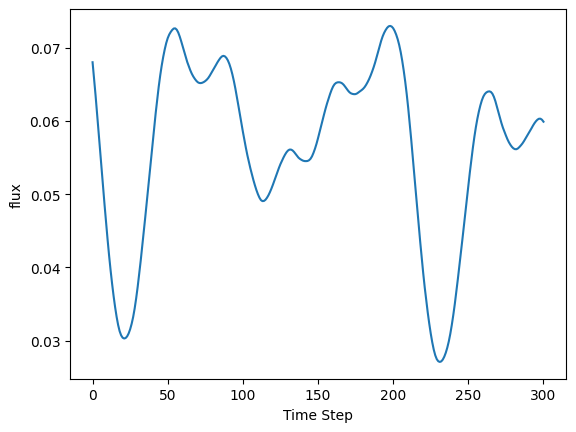
\includegraphics[scale=0.4]{../LightCurveExample.png}
	\end{figure}
\end{frame}
\subsection{Importance of Classifying SOs}
\begin{frame}
	\frametitle{Importance of Classifying SOs}
	Situational Awareness (SSA), the monitering of objects and events in space, has become of
critical to preventing the loss, disruption, and/or degradation of space capabilities and service

\begin{itemize}
	\item
	The classification of SOs is crucial to SSA for:
	\begin{itemize}
		\item
			Collision Avoidance
		\item
			Space Traffic Management
		\item
			Satellite Safety
	\end{itemize}
\end{itemize}
\end{frame}
\subsection{Inverse Lightcurve Problem}
\begin{frame}
	\frametitle{Inverse Lightcurve Problem}
	\begin{itemize}
		\item
			Given observed Lightcurve data we want to infer the properties of SOs
	\end{itemize}

	\begin{block}{InverseLightCurveProblem}
		Let $L = [L_1,L_2,\dots,L_n]$ be an observed lightcurve.

		Let $M$ be a function that maps an unknown set of parameters $SO_\theta$ representing the physical properties of a SO to another vector $\hat{L}\in\mathbb{R}^n$ s.t.

		\[\hat{L} = M(SO_\theta)\]

	We seek $SO_\theta$ s.t. $\hat{L} \approx L$
	\end{block}

	
\end{frame}
\begin{frame}
	\frametitle{Challenges in Finding Solutions to the Problem} 
	Some challenges to finding solutions to this problem are:
	\begin{itemize}
		\item
		Solutions are not unique as a set of SOs may lead to similar matches in modeled and measured lightcurves
		\item
		Uncertianties in measurements and modelling can yield large variations in our solutions
	\end{itemize}
	For these reasons, we consider a data driven approach
	\begin{itemize}
		\item
			We design a Deep Neural Network (DNN) to learn the inverse relationship between Lightcurves and SO properties 
	
	\end{itemize}

\end{frame}
\subsection{K-Nearest Neighbor}
\begin{frame}
	\frametitle{K-Nearest Neighbor (K-NN)}
	The current method for lightcurve classification.
	Computationally expensive...
\end{frame}
\section{CNNs for Lightcurve Classification}
\subsection{Why CNNs?}
\begin{frame}
	\frametitle{Why CNNs?}
	For Lightcurve Classification, CNNs offer a number of benefits over other methods
	\begin{itemize}
		\item
			CNNs are less Computationally expensive
		\item
			Convolutions are great for picking up subtle features in data.
		\item
			CNNs are very well studied for other classification problems so it seems natural to apply it to our problem.
	\end{itemize}
\end{frame}
\subsection{An overview of CNNs}
\begin{frame}
	\frametitle{An Overview of CNNs}

\end{frame}
\subsection{Our Model}
\begin{frame}
	\frametitle{Our Model}
\end{frame}
\section{Training Set Generattion}
\subsection{...}
\begin{frame}
	\frametitle{...}
\end{frame}
\section{Training our Model}
\subsection{...}

\begin{frame}
	\frametitle{...}
\end{frame}
\section{Results}
\subsection{...}
\begin{frame}
	\frametitle{...}
\end{frame}



\end{document} 
